\documentclass[a4paper,12pt]{report}
\usepackage[english,french]{babel}
\usepackage[utf8]{inputenc}
\usepackage[T1]{fontenc}
\usepackage[
    colorlinks=true,
    linkcolor=black,
    citecolor=blue,
    urlcolor=blue
]{hyperref}
\usepackage{amsmath}
\usepackage{amssymb}
\usepackage{amsfonts}
\usepackage{graphicx} 
\usepackage{geometry} 
\geometry{margin=1.2in}
\usepackage{nameref}
\usepackage{csquotes}
\usepackage[backend=biber,style=numeric,sorting=none, autocite=plain, natbib=true]{biblatex}
\addbibresource{ref.bib}
\usepackage{lipsum}
\usepackage{letltxmacro}
\LetLtxMacro{\oldnameref}{\nameref}
\renewcommand{\nameref}[1]{\textbf{\oldnameref{#1}}}
\usepackage{caption}
\DeclareCaptionLabelFormat{boldlabel}{\textbf{#1~#2}}
\captionsetup{
  labelformat=boldlabel,   
  labelsep=period,        
  textfont=small               
}
\usepackage{enumitem}
\setlist[itemize]{label=\textbullet}

\usepackage{array}
\newcolumntype{P}[1]{>{\centering\arraybackslash}p{#1}}

\newcommand{\figref}[1]{Fig.~\ref{#1}}
\newcommand{\tabref}[1]{Tab.~\ref{#1}}


\usepackage[twoside]{fancyhdr}
\setlength{\headheight}{15pt}
\pagestyle{fancy}



% Définir le style fancy normal
\fancyhf{}
\fancyhead[LE,LO]{\leftmark}      % Titre du chapitre sur page paire (gauche)
\fancyhead[RO,RE]{\bfseries \thepage}  % Numéro de page à droite (page impaire)

% Supprimer les en-têtes pour les pages de chapitre
\fancypagestyle{plain}{
  \fancyhf{}  % Vide (ni en-tête ni pied)
  \renewcommand{\headrulewidth}{0pt}  % Pas de ligne d'en-tête
  \renewcommand{\footrulewidth}{0pt}  % Pas de ligne de pied (facultatif)
}

% Assure que les pages de chapitres utilisent le style 'plain'
\renewcommand{\chaptermark}[1]{\markboth{\MakeUppercase{\chaptername\ \thechapter.\ #1}}{}}
\renewcommand{\sectionmark}[1]{\markright{\thesection\ #1}}

% Environnement custom pour abstract (style classique, marges larges)
\newenvironment{customabstract}[1]{%
    \begin{center}
        \bfseries\Large #1\vspace{1em}
    \end{center}
    \begin{quotation}
    \setlength{\leftskip}{1.5cm}
    \setlength{\rightskip}{1.5cm}
}{%
    \end{quotation}
}



\begin{document}

% Title Page
\begin{titlepage}
    \centering
    
\includegraphics[width=0.25\textwidth]{logo/logo_um_2022_filet_noir.png}
    \hspace{1cm}
    
\includegraphics[width=0.28\textwidth]{logo/ssd_logo_couleur_noir_variante_biostats.png}
    \hspace{.9cm}
    
\includegraphics[width=0.25\textwidth]{logo/Faculte-des-Sciences.jpg} \\
    \vspace{2cm}
    \textsc{\Large M2 STATISTIQUES ET SCIENCES DES DONNÉES\\[0.3cm]
        -- BIOSTATISTIQUES --}\\[1.5cm]

    \textsc{\Large Rapport de Stage}\\[0.5cm]
    \rule{\linewidth}{.5pt}\\ [0.4cm]
    \vspace{0.4cm}
    % Title
    {\Huge \bfseries Titre du stage}\\[0.5cm]
    \rule{\linewidth}{.5pt}\\[0.4cm]
    \vspace{0.4cm}
    {\large Guillaume BOULAND}\\[1cm]
    \vspace{0cm}
    \begin{minipage}[t]{0.3\textwidth}
        \vspace{0cm}
        \centering
        \textit{Tuteur académique : }\\[0.2cm]
        \textbf{Nicolas Meyer}
    \end{minipage}
    \hfill
    \begin{minipage}[t]{0.3\textwidth}
        \vspace{0cm}
        \centering
        \textit{Tuteurs professionnels : }\\[0.2cm]
        \textbf{Mai Nguyen-Chi}\\[0.2cm]
        \textbf{Benjamin Charlier}
    \end{minipage}
    \hfill
    \begin{minipage}[t]{0.3\textwidth}
        \vspace{0cm}
        \centering
        \textit{Jury : }\\[0.2cm]
        \textbf{1}\\[0.2cm]
        \textbf{2}\\[0.2cm]
        \textbf{3}
    \end{minipage}




    \vfill
    
\includegraphics[width=0.15\textwidth]{logo/LOGO_CNRS_BLEU.png}
    \hspace{1cm}
    
\includegraphics[width=0.25\textwidth]{logo/logo-lphi-1024x614.png}
    \vspace{1cm}

    {\large \textbf{2023 -- 2024}}
\end{titlepage}

\cleardoublepage
\markboth{Remerciements}{}
\section*{Remerciements}
blabla
\newpage
\cleardoublepage
\markboth{Résumé}{}
\vspace*{\fill}
\begin{customabstract}{Résumé}
    \selectlanguage{french}
    Résumé
\end{customabstract}
\vspace*{\fill}
\newpage
\cleardoublepage
\markboth{Abstract}{}
\vspace*{\fill}
\begin{customabstract}{Abstract}
    \selectlanguage{english}

\end{customabstract}
\vspace*{\fill}
% Table of Contents
\tableofcontents
\newpage


\cleardoublepage
\chapter{Introduction}
\section*{Cadre du stage}
\addcontentsline{toc}{section}{Cadre du stage}
\section*{Contexte}
\addcontentsline{toc}{section}{Contexte}
\section*{Question}
\addcontentsline{toc}{section}{Question}
\section*{Objectifs}
\addcontentsline{toc}{section}{Objectifs}
\chapter{Mactrack2}

\section{Introduction}
Pour répondre à la question biologique posée, nous devions développer un outil qui permettrait de segmenter des macrophages dans des vidéos. POur ce faire, nous avons tout d'abord réfléchi au problème de manière séquentielle, c'est-à-dire image par image. En poursuivant le travail déjà effectué au laboratoire par l'ancien stagiaire Axel de Montgolfier\cite{axel}, étudiant en Master 2 Statistiques et Sciences des Données qui était présent durant l'année 2023-2024, nous avons amélioré le programme MacTrack créé par ses soins, en le rendant plus robuste avec notamment un meilleur jeu de données pour l'entraînement des modèles. Nous pouvons maintenant visualiser la qualité des modèles entraînés. Des scripts plus intuitifs pour les débutants, qui sont la cible de ce projet, ont été ajoutés ainsi qu'une documentation complète sur un site internet, disponible sur le dépôt GitHub du projet (\cite{mactrack2}). Un post-processing a été implémenté pour corriger les erreurs de segmentation des macrophages. Ces erreurs que nous avons rencontrées étaient souvent dues à des problèmes au niveau de l'image de microscopie, comme par exemple la présence d'un fond bruité. Ce process sert aussi pour obtenir une segmentation continue dans le temps, sans changement de numérotation, afin d'obtenir la meilleure analyse possible des flux calciques présent dans ces macrophages.

\chapter{SAM-2}
\section{Introduction}
SAM-2 (\textit{Segment Anything Model 2}) est un modèle de segmentation d'images et de vidéos développé par Meta AI. Il s'agit d'une version améliorée de la première version du modèle, SAM\cite{sam}, généralisant le problème de segmentation d'images au domaine des vidéos (\textit{VOS: Video Object Segmentation}). Entraîné sur plus de 50 000 vidéos pour 600 000 masques (annotations), SAM-2 est capable de segmenter des objets dans des vidéos de manière précise et efficace. L'architecture du modèle (voir \figref{sam2:archi}) est une architecture basé sur les Transformers\cite{Transformer}. Elle comprend un \textit{image encoder} qui est un Vision Transformer hiérarchique appelé Hiera\cite{Hiera}, un \textit{prompt encoder} qui prend en compte des clics (positifs ou négatifs), des boites ou des masques permettant de définir un objet d'intérêt dans une image et un \textit{mask decoder} qui prend ces entrées et en ressort un masque de segmentation de l'objet sélectionné. Il utilise une mémoire en flux (\textit{streaming memory}). Celle-ci permet de traiter les images d'une vidéo en temps réel, une par une. Ainsi, il peut garder en mémoire, à l'aide de la \textit{memory attention} et de la \textit{memory bank}, les objets et leurs interactions au cours du temps, permettant ainsi de générer des masques plus précis et de les corriger en fonction des images précédentes. La \textit{memory attention} permet de \og préparer\fg\ l'image en prenant en compte la \textit{memory bank}, qui garde en mémoire les précédentes images, mais aussi les nouveaux points, masques, boite, que l'utilisateur peut ajouter à chaque image.

\begin{figure}[!ht]
    \centering
    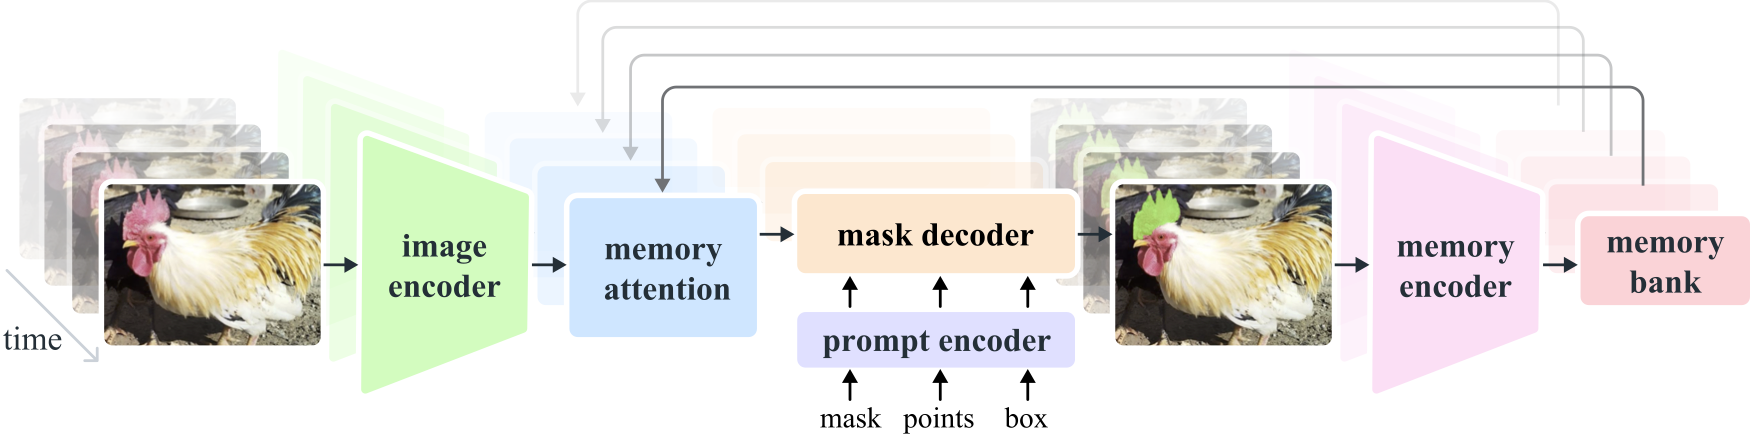
\includegraphics[width=\linewidth]{imgs/model_diagram.png}
    \caption{Architecture de SAM-2 (\textit{figure issue de \cite{sam2}}).}
    \label{sam2:archi}
\end{figure}

Ainsi, SAM-2 est considéré (au même titre que SAM) comme un modèle de fondation (\textit{foundation model})\cite{foundationmodel}, c'est-à-dire un modèle pré-entraîné sur une grande quantité de données, capable de généraliser à de nombreuses tâches différentes. Il est conçu pour être utilisé comme une base pour des tâches de segmentation en gardant de bonnes performances pour l'ensemble des applications de segmentation d'images et de vidéos.

\

Un des problèmes que nous rencontrons avec SAM-2 est que l'utilisateur doit, à la main, sélectionner des objets d'intérêt dans une ou plusieurs images et si durant la vidéo un nouvel objet apparaît, il ne sera pas détecter tant que l'utilisateur ne l'a pas indiqué. Ainsi, nous allons utiliser la génération automatique de masques mise à disposition pour détecter les macrophages de manière automatique sur des images.

performances nulles donc fine tuning



\section{Fine-tuning}
\subsection{Définition}
Le \textit{fine-tuning} (ou \textit{affinage} en français) est une technique d'apprentissage supervisé qui consiste à modifier les poids d'un modèle pré-entraîné sur une tache spécifique. Elle est souvent utilisé pour adapter un modèle généraliste à une tache particulière. Ici, SAM-2 a été entraîné sur des photos qui n'ont rien à voir avec la problématique biologique que nous rencontrons. Par conséquent, afin d'obtenir une bonne segmentation des macrophages, il est nécessaire de modifier les poids du modèle pour obtenir une version spécialisée dans la détection de macrophages. Cela nous évite de devoir entraîner notre propre modèle en partant de rien, ce qui nous demanderait beaucoup trop de données que nous n'avons pas. Mais le nombre de données nécessaires pour obtenir un bon affinage n'est pas négligeable.

Le fine-tuning de SAM-2 agit seulement sur les poids du \textit{prompt encoder} et du \textit{mask encoder}, c'est-à-dire les parties du modèle qui prennent en entrée les points, masques, boites, et qui génèrent les masques de segmentation. Nous spécifions donc la prise en charge des entrées données par l'utilisateur, mais pas la partie qui encode l'image ni la partie qui mémorise les images précédente une fois le fine-tuning fini et que l'on cherche à segmenter une vidéo entière.

\subsection{Jeu de données}
Les annotations sont sous la forme d'images où chaque macrophage est détouré à la main sur le logiciel \textit{ImageJ} (et plus particulièrement \textit{Fiji}\cite{fiji}). Les détourages sont ensuite séparés par label, afin de s'assurer qu'un macrophage ne soit pas confondu avec un autre (\figref{sam2:labels}).

\begin{figure}[!ht]
    \centering
    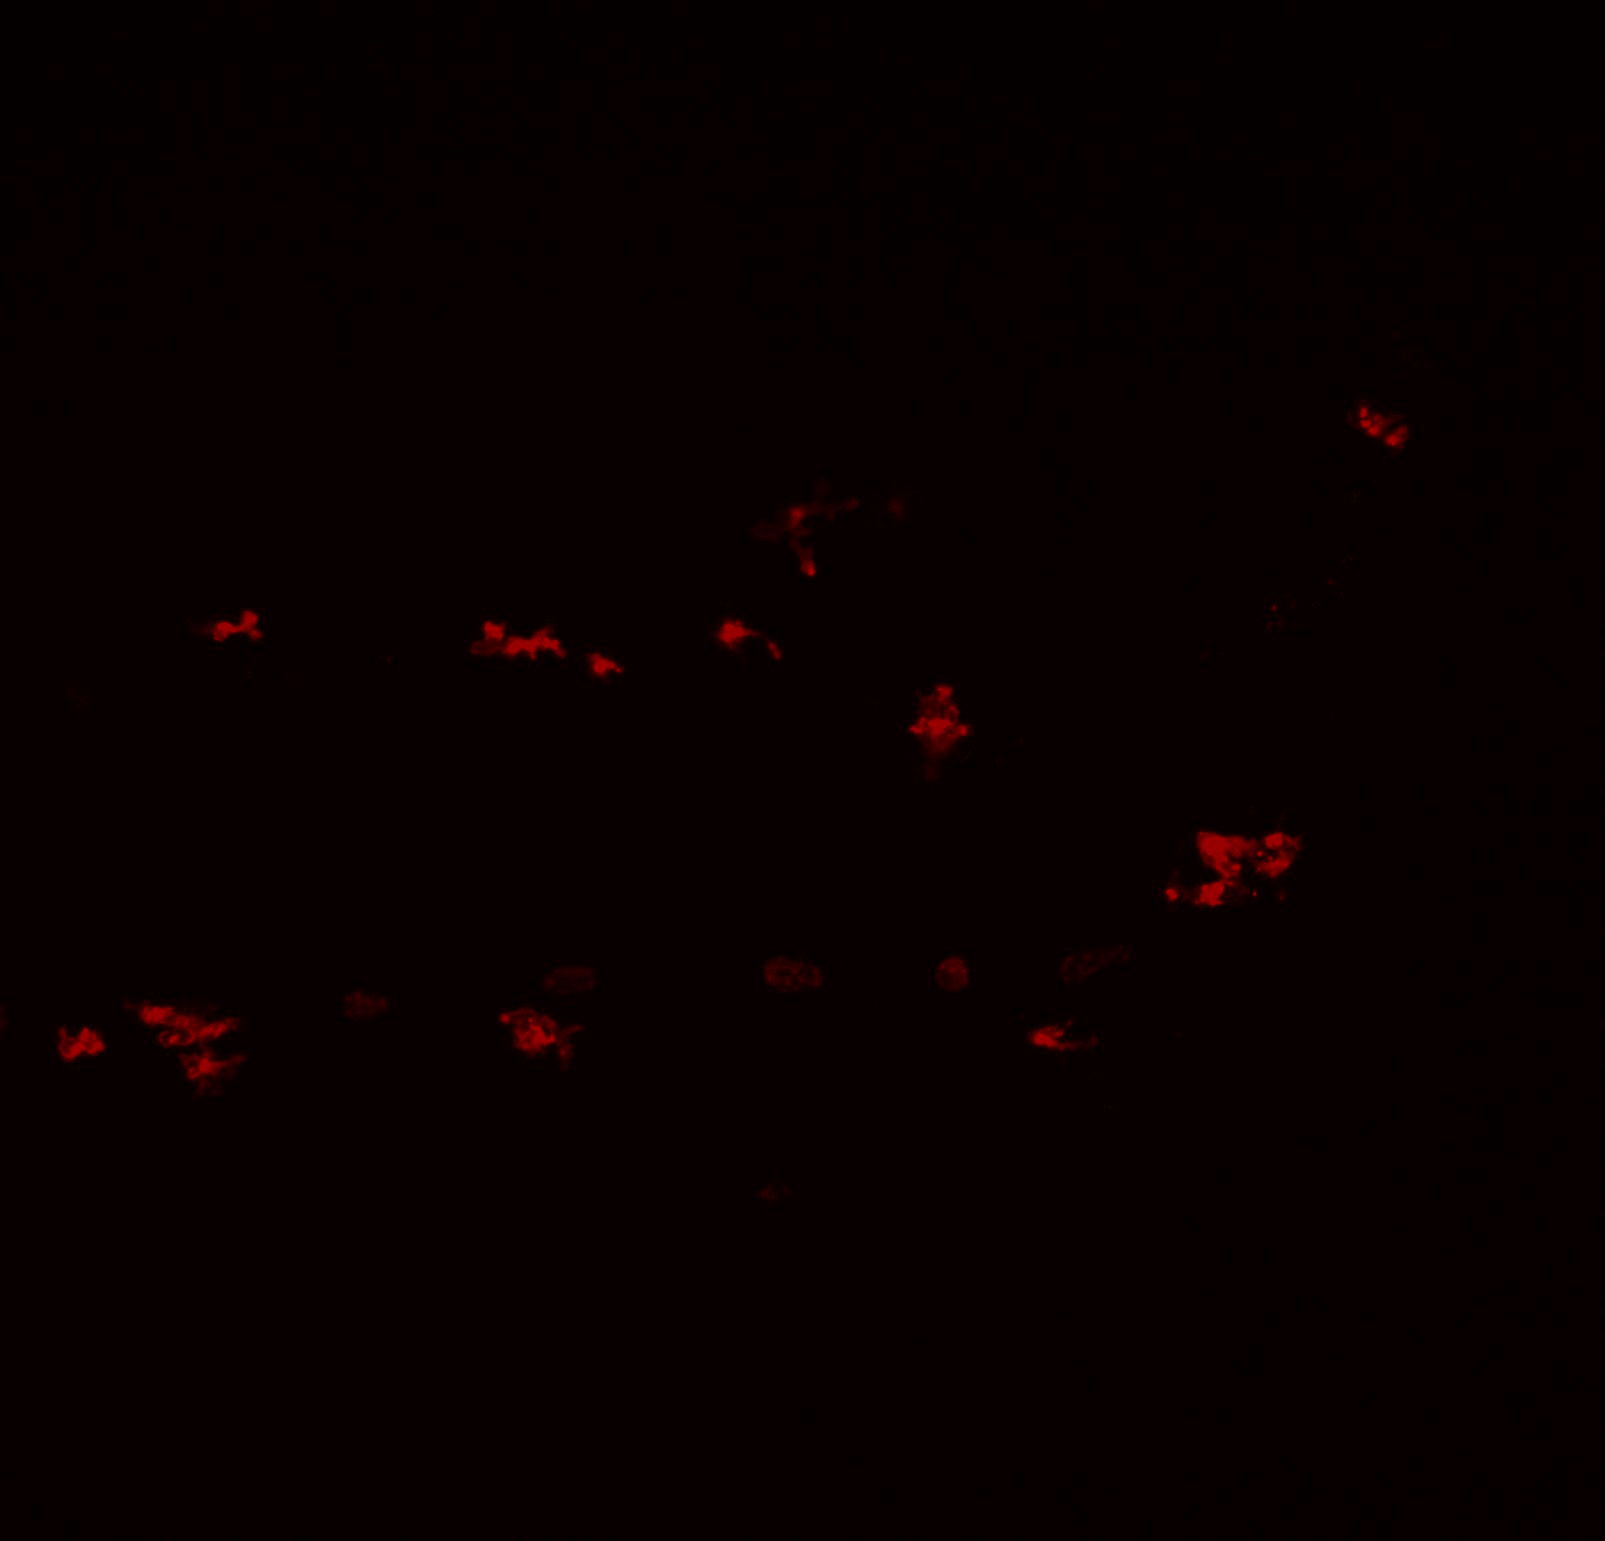
\includegraphics[width=0.4\textwidth]{imgs/001_frame.png}
    \hspace{0.8cm}
    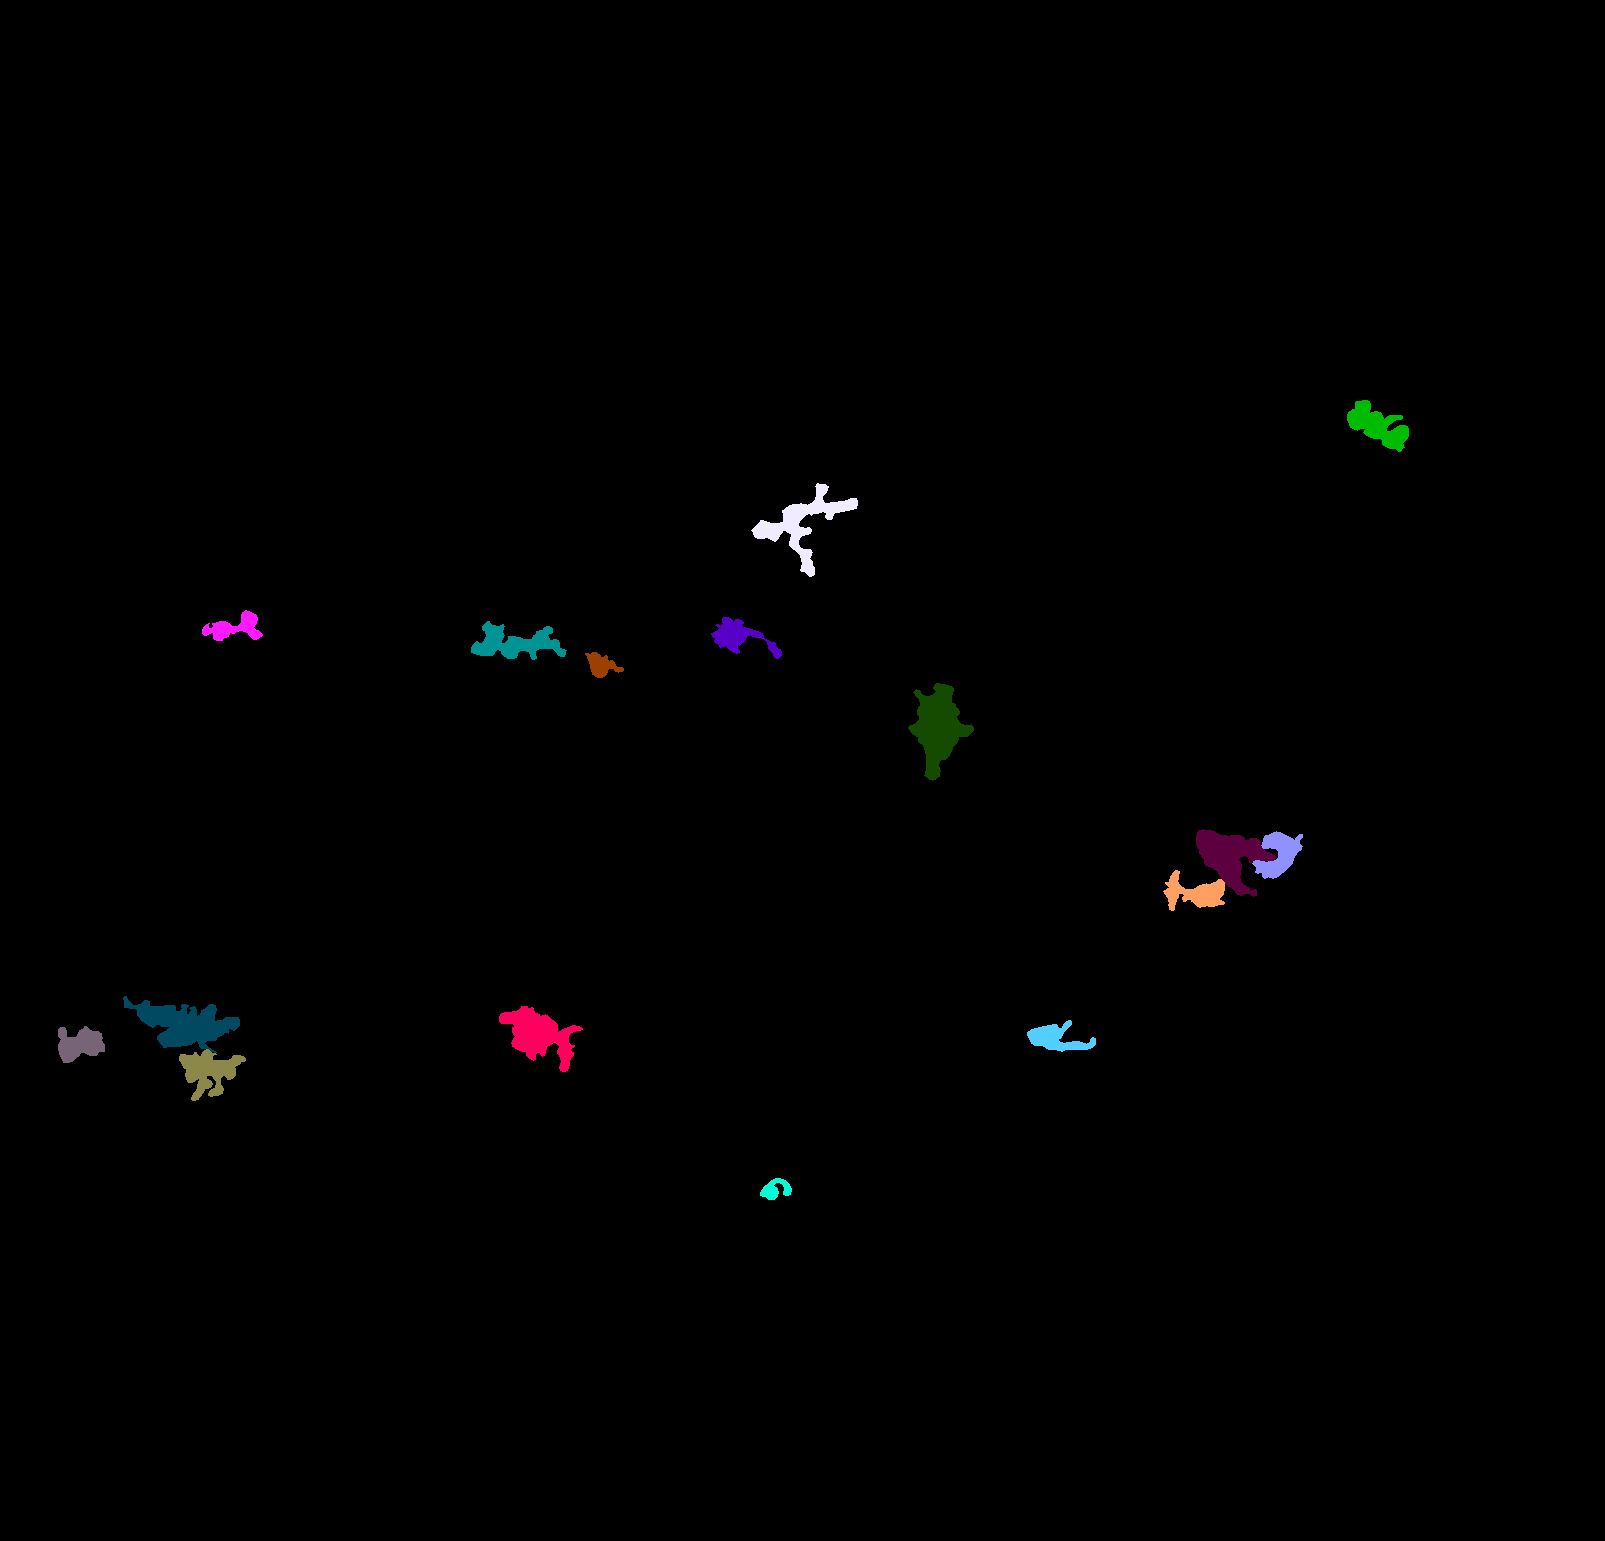
\includegraphics[width=0.4\textwidth]{imgs/001_frame_mask.png}
    \caption{Image d'origine (à gauche) comprenant des macrophages et leur détourage (à droite).}
    \label{sam2:labels}
\end{figure}

\

Malgré que le fine-tuning de SAM-2 ne nécessite pas autant de données que l'entraînement d'un modèle de segmentation complet, il est quand même nécessaire de disposer d'un nombre conséquent de données. Ici, nous avons besoin d'images et de leur segmentation manuelle. Or, le temps imparti pour ce stage ne nous permet pas de composer un jeu de données complet qui satisferait ces besoins. Par conséquent, nous avons utilisé le programme MacTrack2 qui nous a permis de segmenter une vidéo de macrophages. Ainsi, nous disposons de 297 images et masques de macrophages (dont 266 faisant partie d'une seule vidéo) pour ré-entraîner les poids du modèle.

\subsection{Hyper-paramètres}\label{sec:hyperparameters}
Les hyper-paramètres, dans un modèle, constituent les paramètres non appris par le modèle durant l'entraînement (ou le ré-entraînement). Ils sont fixés à l'avance et influencent son comportement et par extension ses performances. Les hyperparamètres du pré-entraînement et de l'entraînement complet de SAM-2 sont disponibles dans leur papier\cite{sam2} page 19.

\

Pour le fine-tuning, les sous-modules affectés sont le \textit{mask decoder} et le \textit{prompt encoder}. Nous utilisons l'optimiseur AdamW\cite{adamw} avec un taux d'apprentissage (\textit{learning rate}) de 0.0001 et une dégradation des poids (\textit{weight decay}) de 0.0001, utile pour la régularisation L2. Le nombre total d'itérations est de 20 000, avec un nombre de pas pour l'accumulation des gradients (\textit{accumulation step}) avant leur mise à jour égal à 4 steps. Le \textit{scheduler}, qui permet de réduire le \textit{learning rate} durant l'entraînement pour améliorer la convergence du modèle. Ici nous utilisons un \textit{stepLR scheduler}, ce qui signifie que tous les $k$ steps, le \textit{learning rate} est multiplié par un facteur $\gamma$. Nous avons $k=500$ et $\gamma=0.1$. Ainsi, le \textit{learning rate} est réduit de 90\% tous les 500 pas (pas vraiment tous les 500 pas, voir la partie suivante).

Contrairement à ce que l'on peut retrouver habituellement dans l'entraînement de modèles, la taille du batch est égale à une seule image. En effet, à chaque pas \dots

\subsection{Fonctions de perte}
Pour entraîner un modèle, il est nécessaire de définir une fonction de perte $\mathcal{L}$ à minimiser. Elle est utilisée pour quantifier la qualité des prédictions du modèle par rapport à la \og vérité\fg (ground truth). Dans le cas du fine-tuning de SAM-2, nous utilisons une combinaison de deux fonctions de perte : la \textit{binary cross-entropy loss} qui sert de perte pour la segmentation et la \textit{score loss} qui est utilisée en complément pour évaluer la qualité des prédictions des masques à partir de la métrique IoU (\textit{Intersection over Union}). L'IoU est une métrique grandement utilisée dans les problèmes de segmentation d'images. Elle est définie, pour un macrophage $k$ dans une image, de la manière suivante et peut être illustrée par la \figref{sam2:iou} :
$$\text{IoU}(M_k, G_k) = \frac{\lvert M_k \cap G_k\rvert}{\lvert M_k \cup G_k\rvert}= \frac{\displaystyle\sum_{i,j}M_k[i,j]\cdot G_k[i,j]}{\displaystyle\sum_{i,j}M_k[i,j]+ \displaystyle\sum_{i,j}G_k[i,j] - \displaystyle\sum_{i,j}M_k[i,j]\cdot G_k[i,j]}$$

\noindent avec :
\begin{itemize}
    \item $i\in \{1, \ldots, H\}$ et $j\in \{1, \ldots, W\}$ la hauteur et la largeur respectivement de l'image,
    \item $M_k = \left(M_k[i,j]\right)_{i,j}$ le masque prédit pour l'objet $k$, une matrice binaire de taille $H\times W$ où chaque pixel vaut 1 s'il est dans le masque prédit, c'est-à-dire que si la probabilité que le pixel $(i,j)$ appartienne au masque de l'objet $k$ est supérieure à $0.5$, sinon il vaut 0. On a donc :
          $$M_k[i,j] = \begin{cases}
                  1 & \text{si } p > 0.5, \\
                  0 & \text{sinon}.
              \end{cases}$$
          avec $p$ la probabilité que le pixel $(i,j)$ appartienne au masque de l'objet $k$,
    \item $G_k=\left(G_k[i,j]\right)_{i,j}$ le masque de vérité pour l'objet $k$, une matrice binaire de taille $H\times W$ où chaque pixel (élément de la matrice) vaut 1 s'il est dans le masque de vérité, sinon il vaut 0,
    \item $\lvert M_k \cap G_k\rvert = \sum_{i,j}M_k[i,j]\cdot G_k[i,j]$ l'intersection entre le masque prédit et le masque de vérité, autrement dit le nombre de pixels en commun entre les deux masques,
    \item $\lvert M_k \cup G_k\rvert = \sum_{i,j}M_k[i,j]+ \sum_{i,j}G_k[i,j] - \sum_{i,j}M_k[i,j]\cdot G_k[i,j] $ l'union entre le masque prédit et le masque de vérité, autrement dit le nombre de pixels dans au moins un des deux masques,
    \item $\sum_{i,j}M_k[i,j]$ le nombre de pixels du masque prédit,
    \item $\sum_{i,j}G_k[i,j]$ le nombre de pixels du masque de vérité.
\end{itemize}

\begin{figure}[!ht]
    \centering
    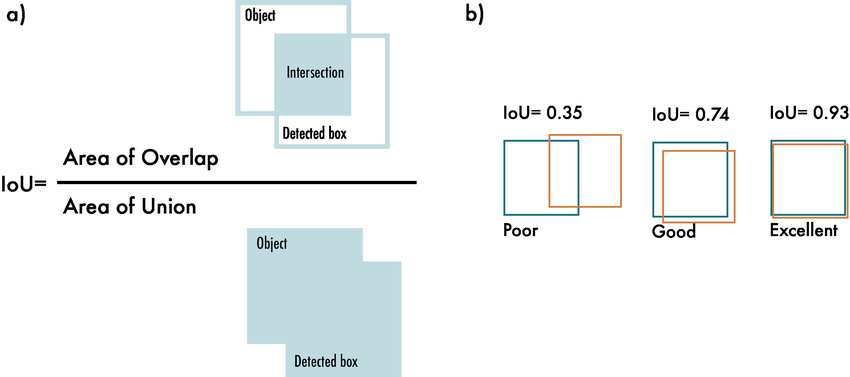
\includegraphics[width=.8\linewidth]{imgs/iou.png}
    \caption{Schématisation de l'IoU (figure issue de \cite{iou}).}
    \label{sam2:iou}
\end{figure}

En moyennant sur tous les objets $k$ d'une image, on obtient la mIoU (IoU moyenne), métrique très utilisée, pour cette image :
$$\text{mIoU} = \frac{1}{K}\sum_{k=1}^{K}\text{IoU}(M_k, G_k)$$

Ainsi, nous pouvons définir la \textit{score loss} comme suit :
$$\mathcal{L}_{\text{score}} = \frac{1}{K}\displaystyle\sum_{k=1}^{K}\lvert s_k - \text{IoU}(M_k, G_k)\rvert$$
\noindent avec $K$ le nombre total de masques (donc de macrophages ou d'objets) dans l'image et $s_k$ le score prédit pour l'objet $k$ à partir de $M_k$.

Nous comparons donc le score prédit par le modèle pour chaque masque à la véritable qualité de chacun d'eux (l'IoU). Puisque'on cherche à minimiser cette perte, on aimerait que pour tout $k$, $s_k\simeq \text{IoU}(M_k,G_k)$ pour que la perte soit proche de 0.

Si $K=0$, alors cela signifie qu'il n'y a pas de masques dans l'image, donc pas de macrophages. Un tel cas peut être rencontré, mais nous avons décidé de ne pas l'inclure dans le fine-tuning, car il n'apporte pas d'information utile concernant la segmentation des macrophages.

\

D'un autre côté, la \textit{binary cross-entropy loss} $\mathcal{L}_{BCE}$ est une fonction de perte généralement utilisée dans des problèmes de classification binaire, et notamment dans les problèmes de segmentation d'images. Elle est utilisée pour quantifier la différence entre les prédictions du modèle et les véritables annotations (masques de vérité). Elle est définie comme suit :

$$\mathcal{L}_{BCE} = -\frac{1}{K\times H\times W}\displaystyle\sum_{k=1}^{K}\sum_{i=1}^{H}\sum_{j=1}^{W}y_{k,i,j}\log\hat{y}_{k,i,j} + (1-y_{k,i,j})\log(1-\hat{y}_{k,i,j})$$
avec :
\begin{itemize}
    \item $y_{k,i,j}\in\{0,1\}$ la valeur du pixel $(i,j)$ du masque de vérité pour l'objet $k$. On peut notamment remarquer que la matrice $G_k=\left(y_{k,i,j}\right)_{i,j}$ est une matrice binaire (composée de 0 et de 1) de même dimension que les dimensions de l'image ($H\times W$).
    \item $\hat{y}_{k,i,j}\in\left[0,1\right]$ est la probabilité que le pixel $(i,j)$ appartienne au masque de l'objet $k$. Elle est obtenue par la transformation sigmoïde appliquée à la prédiction des masques du modèle, qui sont des logits générés par le \textit{mask decoder} (voir \tabref{sam2:logit}). On a donc :
          $$\hat{y}_{k,i,j} = \sigma(z_{k,i,j}) = \frac{1}{1+\exp(-z_{k,i,j})}$$\\
          avec $z_{k,i,j}$ le logit du pixel $(i,j)$ du masque prédit pour l'objet $k$.

          \begin{table}[!ht]
              \centering
              \renewcommand{\arraystretch}{1.5}
              \begin{tabular}{|c|P{8cm}|c|}
                  \hline
                  \textbf{Logit} $(z_{k,i,j})$ & \textbf{Interprétation}                        & \textbf{Sigmoid} $(\hat{y}_{k,i,j}) $ \\
                  \hline
                  $+10 $                       & Très sûr qu'il s'agit d'un objet               & $\approx 1$                           \\
                  $+1$                         & Assez confiant qu'il s'agit d'un objet         & $\approx 0.75$                        \\
                  $0$                          & Incertitude totale                             & 0.5                                   \\
                  $-1$                         & Assez confiant qu'il s'agit du fond de l'image & $\approx 0.25$                        \\
                  $-10$                        & Très sûr qu'il s'agit du fond de l'image       & $\approx 0$                           \\\hline
              \end{tabular}
              \caption{Différents exemples des valeurs que peuvent prendre les sorties du \textit{mask decoder} (logits), leur interprétation et la valeur de la probabilité associée (par transformation sigmoïde).}
              \label{sam2:logit}
          \end{table}
    \item $H$ et $W$ la hauteur et la largeur de l'image.
    \item $K$ le nombre total de masques (donc de macrophages ou d'objets) dans l'image.
\end{itemize}

\

Interprétations fonction de perte \dots
ressemble a kullbackleibler mias différences \dots

\

Finalement, la fonction de perte totale est une combinaison de ces deux dernières :
$$\mathcal{L} = \mathcal{L}_{BCE} + \lambda\mathcal{L}_{\text{score}}$$
\noindent avec $\lambda$ un hyper-paramètre qui permet de pondérer l'importance de la \textit{score loss} par rapport à la \textit{binary cross-entropy loss}. Dans notre cas, nous avons fixé $\lambda$ à $0.05$.

\subsection{Optimisation}
Une fois la perte calculée, elle est divisée par le nombre de pas d'accumulation des gradients, soit 4 dans notre cas, comme défini dans la partie~\ref{sec:hyperparameters} introduisant les hyper-paramètres. Cela nous permet d'éviter de multiplier le gradient total par ce facteur. C'est utilisé lorsque l'on accumule des gradients sur plusieurs images (ici 4 fois une image) pour que la somme finale corresponde en réalité à une moyenne sur ce batch étendu. Ainsi, nous simulons un batch de taille 4 alors qu'en réalité nous n'avons qu'une seule image par step.

Ensuite, les gradients sont calculés en utilisant la méthode \textit{backward} du package PyTorch\cite{pytorch}, à partir de la perte totale $\mathcal{L}$ divisée par cet \textit{accumulation step}. Puis, tous ces 4 steps, nous mettons à jour l'optimiseur AdamW. Puisque le nombre de pas avant la mise à jour du \textit{learning rate} est de 500, il faut en réalité 2000 itérations avant de le mettre à jour. Ainsi, le \textit{learning rate} est réduit de 90\% tous les 2000 pas, et non tous les 500 pas comme introduit dans la partie~\ref{sec:hyperparameters}. Ensuite, les gradients sont remis à zéro pour le prochain pas d'accumulation.

Pour finir, nous calculons l'IoU moyenne au pas $\ell$ comme étant :

$$\text{mIoU}_\ell = \begin{cases}
        0.9\cdot \text{mIoU}_{\ell-1} + 0.1\cdot \frac{1}{K}\sum_{k=1}^{K}IoU(M_k,G_k) & \text{si } k > 0, \\
        0                                                                              & \text{sinon.}
    \end{cases}
$$

\subsection{Résultats et comparaisons}
graphes miou et loss avant division par accumulation step


\section{Propagation dans une vidéo}

\chapter{Conclusion}
\section*{Disponibilité du code}
Le code de MacTrack2 est disponible, ainsi que deux scripts détaillés pour la création de modèle et l'analyse d'une vidéo, avec un jeu de données d'exemple pour chacun des deux scripts, à l'adresse suivante : \url{https://github.com/guibouland/MacTrack2}.\\

Un site internet est disponible sur ce dépôt GitHub, regroupant toute la documentation et des instructions détaillées pour les utilisateurs plus novices, notamment les biologistes traitant la même problématique, qui sont la cible principale de ce projet. Il servira aussi aux futurs membres du laboratoire LPHI qui souhaitent utiliser MacTrack2 pour leurs propres projets.

\chapter{Matériel et Méthodes}\label{matmeth}
tests tests\cite{cortacero2023evolutionary,sam,sam2,adamw}
\section*{Acquisition des images}
microscope \dots norma merci
\section*{Fine-tuning de SAM-2}
L'optimiseur AdamW a été utilisé avec comme hyper-paramètres un taux d'apprentissage (\textit{learning rate}) de 0.0001, une dégradation de pondération (\textit{weight decay}) de 0.0001.
L'entraînement a été effectué avec 20000 itérations. Nous avons utilisé un GPU Nvidia A10 Tensor Core avec 24 Go de mémoire.


\newpage

\printbibliography
\end{document}